\documentclass[border=10pt]{standalone}
\usepackage{pgfplots}
\pgfplotsset{compat=1.18}
\begin{document}
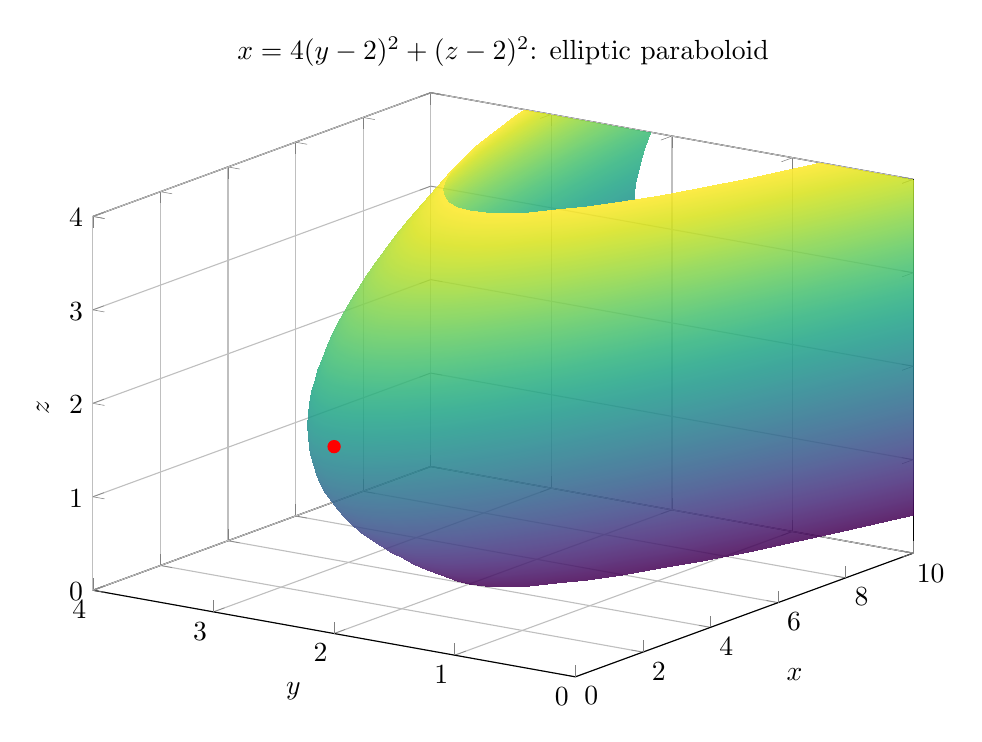
\begin{tikzpicture}
\begin{axis}[
    width=12cm,
    height=9cm,
    view={-55}{22},
    xlabel=$x$, ylabel=$y$, zlabel=$z$,
    title={$x=4(y-2)^2+(z-2)^2$: elliptic paraboloid},
    domain=0:4,
    y domain=0:4,
    samples=35,
    samples y=35,
    colormap/viridis,
    grid=major,
    zmin=0, zmax=4,
    xmin=0, xmax=10,
    ymin=0, ymax=4,
]
\addplot3[surf,shader=interp,opacity=0.85]
({4*(y-2)^2+(x-2)^2}, y, x);
\addplot3[only marks, mark=*, mark size=2.2pt, red]
coordinates {(0,2,2)};
\end{axis}
\end{tikzpicture}
\end{document}